\documentclass{standalone}
\usepackage{tikz}
\usetikzlibrary{quantikz}

\begin{document}

\begin{tikzpicture}[scale=0.8]
    % Draw the main lines
    \draw[thick] (-0.5,-1) -- (6.5,-1);
    \draw[thick] (-0.5,-2) -- (6.5,-2);
    \draw[thick] (-0.5,-3) -- (6.5,-3);
    \draw[thick] (-0.5,-4) -- (6.5,-4);

    % Draw the dashed box and label
    \draw[dashed] (-0.5,-1) -- (-0.5,-4);
    \draw[dashed] (6.5,-1) -- (6.5,-4);
    \draw[dashed] (-0.5,-1) -- (6.5,-1);
    \draw[dashed] (-0.5,-4) -- (6.5,-4);
    \node at (7,-2.5) {$\times D$};

    % Draw the rotation gates
    \node[scale=1.2] at (-0.5,-1) {\textcolor{red}{$R_y(\theta_1)$}};
    \node[scale=1.2] at (-0.5,-2) {\textcolor{red}{$R_y(\theta_2)$}};
    \node[scale=1.2] at (-0.5,-3) {\textcolor{red}{$R_y(\theta_3)$}};
    \node[scale=1.2] at (-0.5,-4) {\textcolor{red}{$R_y(\theta_4)$}};

    % Draw the Hadamard gates
    \node[scale=0.8] at (3.5,-1) {\textcolor{blue}{$\oplus$}};
    \node[scale=0.8] at (3.5,-2) {\textcolor{blue}{$\oplus$}};
    \node[scale=0.8] at (3.5,-3) {\textcolor{blue}{$\oplus$}};
    \node[scale=0.8] at (3.5,-4) {\textcolor{blue}{$\oplus$}};

    % Draw the measurement nodes
    \node[circle, fill=black, scale=0.5] at (5.5,-1) {};
    \node[circle, fill=black, scale=0.5] at (5.5,-2) {};
    \node[circle, fill=black, scale=0.5] at (5.5,-3) {};
    \node[circle, draw=black, thick, scale=0.5] at (5.5,-4) {};

    % Draw the control lines
    \draw[thick] (1.5,-1) -- (4.5,-1);
    \draw[thick] (1.5,-2) -- (4.5,-2);
    \draw[thick] (1.5,-3) -- (4.5,-3);
    \draw[thick] (1.5,-4) -- (4.5,-4);

    % Add the description text
    \node [below right] at (7,-2.5) {\small{An example of BasicEntangler ansatz. $R_y(\theta_i)$ is a rotation gate around the y-axis by an angle $\theta_i$ applied to the i-th qubit, where $i=1,2,3,4$. The circuit layer in the dashed box can be repeated $D$ times to increase the representational capacity of the ansatz.}};
\end{tikzpicture}

\end{document}